% Prof. Dr. Ausberto S. Castro Vera
% UENF - CCT - LCMAT - Curso de Ci\^{e}ncia da Computa\c{c}\~{a}o
% Campos, RJ,  2021
% Disciplina: Paradigmas de Linguagens de Programa\c{c}\~{a}o



\chapter{ Conceitos b\'{a}sicos da Linguagem JavaScript}

Neste cap\'{\i}tulo \'{e} serão apresentados os principais conceitos da linguagem JavaScript, sua estrutura léxica, operadores, laços de repetição entre outros tópicos.
Os livros b\'{a}sicos e recomendados o estudo da Linguagem JavaScript s\~{a}o: \cite{flanagan2020javascript}, \cite{powers2015javascript} entre outros.


\section{Estrutura Léxica}
A linguagem JavaScript é feita utilizando o set de caracteres Unicode, que dá suporte a praticamente todas as linguagens utilizadas
atualmente no mundo. Essa é uma linguagem case sensitive, ou seja, os nomes de variáveis, funções e outros identificadores devem ser sempre utilizados de maneira consistente, ao contrário do que acontece no html, por exemplo. %Necessário melhorar +/-
Além disso, o JavaScript ignora os espaços e as quebras de linha, com algumas exceções. Isso permite que os programas sejam identados de maneira que façam o código ser legível e fácil de entender.
Falando em tornar o código legível, os comentários em JavaScript podem ser feitos de duas formas: uma delas são os comentários de uma só linha, que utilizam "//" e a outra são os comentários de múltiplas linhas, que ignorarão tudo que está dentro dos caracteres.
Observe o exemplo abaixo:
\newline
\begin{lstlisting}[language=JavaScript]
/*  Explicacao do codigo
	O codigo abaixo realiza... */
var helloWorld = function(){
	console.log('Hello World!');
}
helloWorld();
\end{lstlisting}
*No JavaScript o uso de vírgulas é opcional.
 


   \begin{figure}[H]
    \begin{center}
        \caption{Melhores Livros} \label{livros}
        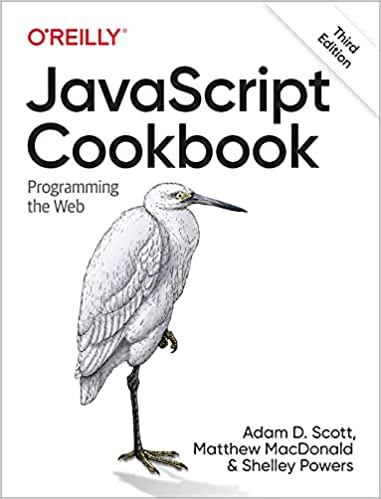
\includegraphics[width=6cm]{2021} 
                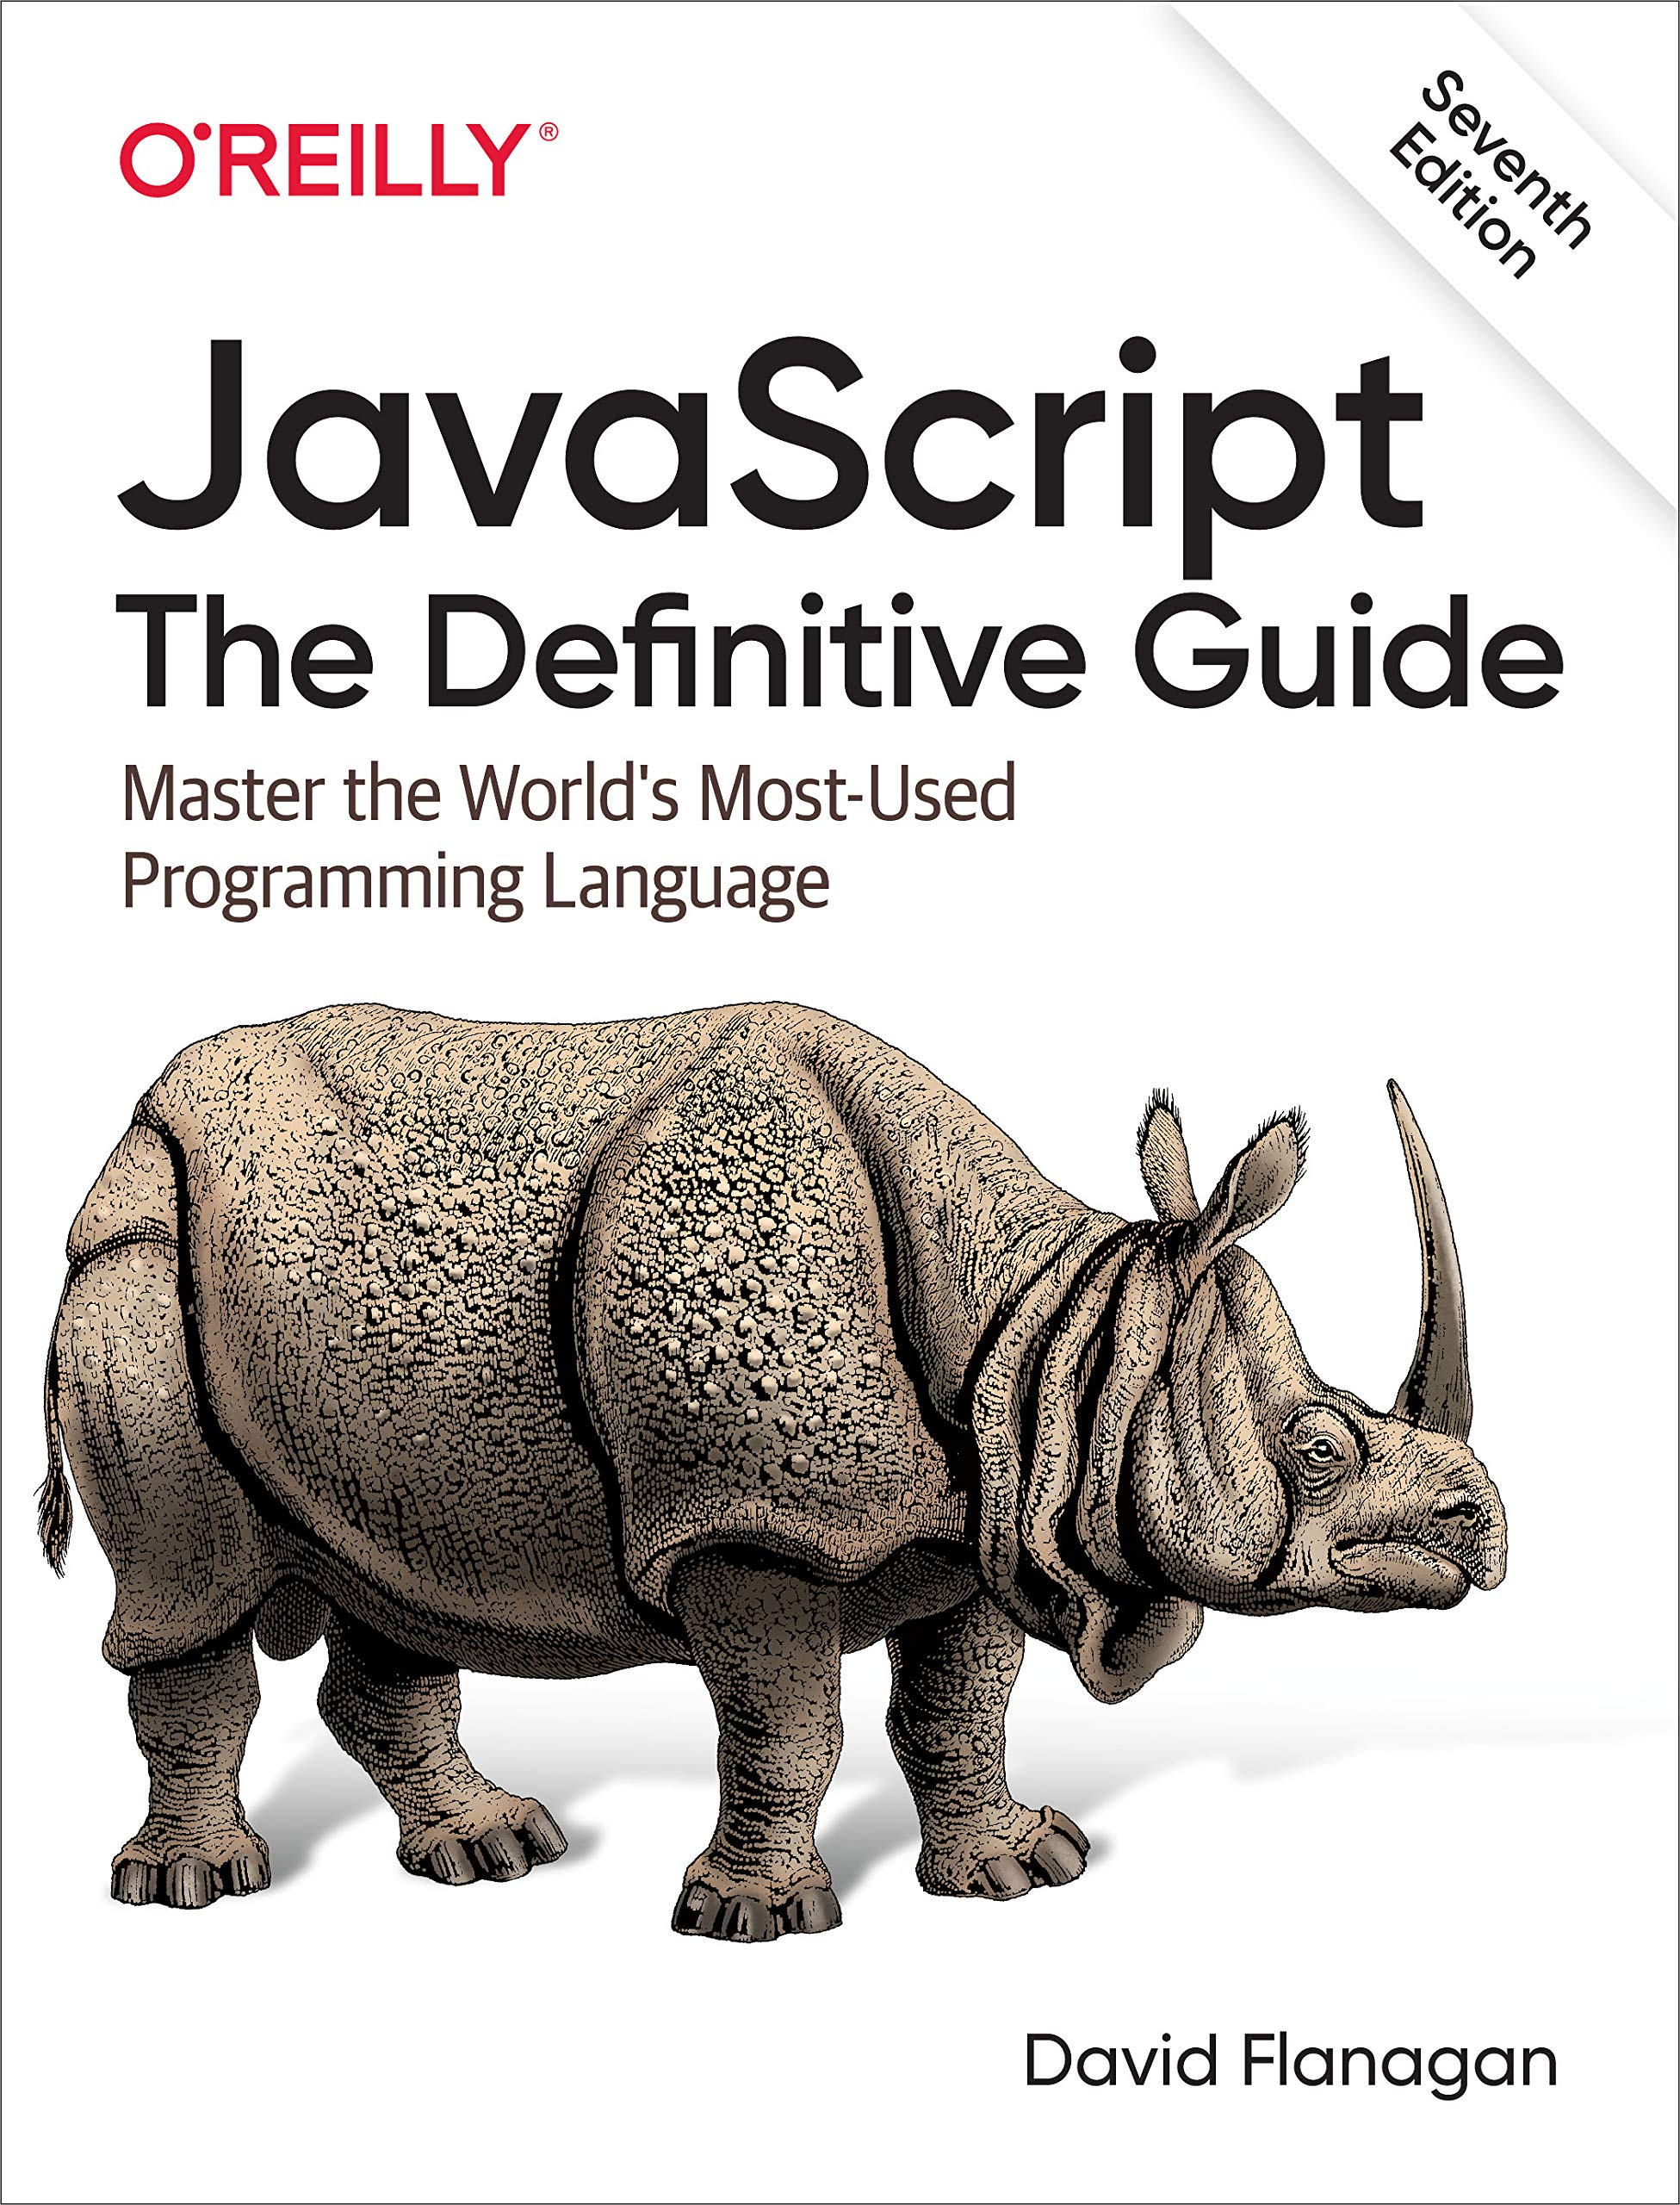
\includegraphics[width=6cm]{2020b}
        {\tiny \sf Fonte: O autor }
    \end{center}
   \end{figure} 
    %%%%%%%%=================================
    \section{Operadores}
    A linguagem JavaScript tem operadores
    \begin{lstlisting}
    ++								//incremento
    --								//decremento
    !								//inverte valores em booleano
    ==								//testa equalidade
    !=								//testa inequalidade
    !==								//testa inequalidade de forma rigorosa (mesmo tipo e valor)
    //testa por equalidade estrita, ou seja, o tipo tambem tem que ser o mesmo
    ===	
    ||								//OR
    &&								//AND
    =								//Atribui um valor a uma variavel
    *=, /=, %=, +=...				//Faz uma atribuicao e um calculo
    //Menor que, maior que, menor ou igual que, maior ou igual que
    <, >, <=, >=
    \end{lstlisting}
    \section{Vari\'{a}veis e Constantes}
    %%%%%%%%=================================
    Com base no livro\cite{flanagan2020javascript}, uma variável é, de forma resumida, um nome simbólico para um valor armazenado no computador. Quando chamamos uma variável, estamos acessando o valor guardado por ela. 
   	\par Na linguagem JavaScript, existem dois tipos de variáveis: as primitivas e as de objeto. 
    Para se declarar uma no JavaScript é necessário utilizar a palavra reservada "var" ou "let" seguida de seu nome. A linguagem automaticamente detectará o tipo, sem ser necessário especificá-lo com antecedencia, o que é o caso em linguagens como C e Java. Abaixo encontram-se exemplos da declaração de variáveis no JavaScript:
    \newline
    
    \begin{lstlisting}
    //E possivel declarar uma variavel vazia
    var a;
    var b = 100;
    var name = "Lucas";
    
    //Tambem e possivel declarar multiplas variaveis numa so linha
    var A = 0, B = 1, C = 2;
    
    //Variaveis tambem podem ser criadas dentro de lacos de repeticao
    (for var i = 0; i<10; i++){
    	console.log(i)
    }
    \end{lstlisting}
    
    \subsection{Tipos Primitivos}
    
	Os tipos primitivos do JS incluem números, strings de textos e valores booleanos (true e false).
	Além disso, existem também os tipos especiais "null" e "undefined", que são valores primitivos, porém não são números, strings ou booleanos. Nesse sentido, cada um é considerado membro de um tipo especial.  
	\subsubsection{Números}
	%TALVEZ Desconsiderar essa subsection
	Uma fator da linguagem JavaScript que é incomum em outras línguas é que não há distinção entre inteiros e floats, sendo todos os números representados como floats. 
	A linguagem armazena os números utilizando o formato de floats de 64 bits, podendo armazenar números grandes com precisão considerável.
	
	\subsubsection{Strings}
	De acordo com \cite{flanagan2020javascript}, uma string é uma sequência imutável de valores de 16 bits, onde cada um representa geralmente um caractere Unicode. O tamanho da string dependerá de quantos desses valores ela contém. Para incluir uma string num programa, basta colocar aspas (simples ou duplas). Por exemplo:
	\newline
	
	\begin{lstlisting}
	//E uma string vazia
	''
	
	"10.24"	
	//Utilizacao da combinacao de aspas simples e duplas
	'O numero "8" e par'				
	
	mensagemOla = "Ola, seja bem vindo" 
	//Printa o conteudo da variavel no console do navegador
	console.log(mensagemOla)	
	
	/*compara o valor da variavel e retorna true ou false. 
	No caso, retornara true*/
	a = "Ola"
	a == "Ola"
	
	
	\end{lstlisting}
	
	\subsubsection{Booleanos}
	Conforme \cite{powers2015javascript}, um valor booleano é um valor que representa verdade ou falsidade. Deste modo, só há dois possíveis valores para um booleano. No JavaScript, as palavras reservadas para os booleanos são "true" e "false", e são geralmente o resultado de uma comparação. Observe o exemplo:
	\newline
	
	\begin{lstlisting}
		a = 10
		b = 3
		a == b
		false
		
		a == 10
		true
	\end{lstlisting}
	\subsubsection{Tipos Especiais}
	Consoante a \cite{flanagan2020javascript}, "null" é uma palavra reservada que geralmente indica ausência de um valor. Se utilizarmos o comando "typeof" no "null", veremos que será retornado "object", o que significa que "null" é algo que indica a ausência de objeto. Resumindo, pode ser utilizado para indicar que não há valor em uma variável, string ou objeto. 
	
	Por isso, "null" e "undefined" costumam ser definidos como um único objeto do seu tipo.
	
	
	\subsection{Tipos de Objeto}
	Segundo \cite{flanagan2020javascript}, qualquer valor que não seja um número, string, objeto ou null e undefined é um objeto, ou seja, é uma coleção de propriedades onde cada uma tem um nome e valor.
	
	\subsubsection{Globais}
	Os objetos globais são aqueles que podem ser usados em todo programa escrito em JavaScript. Quando um interpretador da linguagem inicia, ele cria novos objetos globais e os dá as propriedades que o definem. 
	Algumas das propriedades globais existente são: undefined, Infinity, NaN.
	Além de propriedades e funções globais, no JavaScript existem também constructor functions, como: Date(), Object() e objetos globais, como o Math e JSON.
	
	São exemplos de funções globais: 
	\newline
	\begin{lstlisting}
	isNan()			  	//Retorna se um valor e um numero ou nao.
	parseInt()		  //Recebe o conteudo de uma string e converte para. inteiro
	parseFloat() 	  //Recebe uma string e a converte para float.
	eval()	  		  //Avalia codigo representado por uma string.
	isFinite()		  //Verifica se um numero e finito.
	
	\end{lstlisting}
	
	
	\section{Estrutura de Controle e Funções}
	De acordo com \cite{flanagan2020javascript}, uma estrutura de controle dita a ordem em que instruções serão execudas. Estruturas muito conhecidas em outras linguagens estão presentes também no JavaScript.
	
	\subsection{O comando IF}
	O comando IF funciona para fazer com que o JavaScript execute expressões condicionalmente. Isso significa que o computador somente executará uma determinada instrução caso a condição seja verdadeira. Caso a seja falsa, o programa executará outro do bloco de código.
	O comando IF na linguagem toma a seguinte forma:
	\newline
	
	\begin{lstlisting}
		//Sintaxe
		if(condicao){
			//realiza instrucao A
		}else{
			//realiza outra instrucao
		}
		
		//-----Exemplo-----
		var nome = "Marcos"
		
		if(nome == Marcos){
			console.log("Bem vindo, Marcos!")
		}else{
			console.log("Apenas Marcos pode ler esta mensagem!")
		}
	\end{lstlisting}
	
	É possível também utilizar IFs dentro de outros IFs, como no exemplo abaixo:
	\newline
	\begin{lstlisting}
	
		if(animal == cachorro){
			console.log("Um cachorro e um animal")
			if(cachorro == panda){
				console.log("Um panda e um cachorro)
			}else{
				console.log("Um panda nao e um cachorro")
			}
		}
		
	\end{lstlisting}
	
	\subsection{Laços de Repetição}
	Laços de repetição executam uma instrução até que uma determinada condição seja verdadeira. Na linguagem JavaScript, os laços de repetição são o 'while', 'do ... while' e o 'for'.
	\newline
	\newline
	
	\subsubsection{While}
	Os laços de repetição "while" tem a seguinte sintaxe no JavaScript:
	\newline
	\begin{lstlisting}
		while(condicao == true){
			execute...
		}
		
		//O progrma abaixo conta de 0 a 999
		vai i = 0;
		
		while(i < 1000){
			console.log(i)
			i++
		}
		
	\end{lstlisting}
	É importante que o laço "while" atinga em algum momento uma condição de saída. Caso contrário, o programa continuará executando indefinidamente. No exemplo abaixo, temos um programa sem condição de saída.
	\newline
	\begin{lstlisting}
		while(Bolsonaro == Horroroso){
			console.log("O presidente e horroroso")
		}
		//O programa printara a mensagem acima indefinidamente
	\end{lstlisting}
	
	\subsection{For}
	
	Geralmente, os laços que utilizam o "for" são mais simples de serem lido. Isso devido ao fato de poderem executar uma variável inicial, testá-la e incrementála em uma única linha. Na linguagem, o laço for funciona com a seguinte sintaxe:
	\newline
	\begin{lstlisting}
		for(inicia variavel; testa condicao; incrementa){
			realiza instrucao
		}
	
	 	//-------Exemplo-------
	 	//O programa abaixo calcula fatoriais
	 	var fatorial = 10;
	 	var resultado = fatorial;
	 	var multiplicadorInicial = fatorial - 1
	 	
	 	for(var i = multiplicadoInicial; i > 1; i--){
	 		resultado = resultado * i;
	 	}
	 	
	 	console.log(resultado)
	 	
	\end{lstlisting}
	
	\subsection{Do ... While}
	
	Ao contrário do "while" e do for, o "dowhile" verifica a condição apenas no final da função. A sintaxe do "dowhile" no JavaScript é a listada abaixo:
	\newline
	\begin{lstlisting}
	do
		instrucao
	while(condicao == true)
	
	//-------EXEMPLO-------
	//O programa abaixo conta de 1 a 100
	var i = 0;
	do
		i++
		console.log(contador)
	while(i<100)
	
	\end{lstlisting}
	
	Caso o código acima fosse executado com o "while", o programa contaria apenas de 1 a 99, já que a checagem no início impediria o programa de fazer mais uma iteração.
	
	 
	




